\documentclass[12pt]{article}

\setlength{\topmargin}{0pt}
\setlength{\textheight}{9in}
\setlength{\headheight}{0pt}
\setlength{\headsep}{0pt}
\setlength{\oddsidemargin}{0.25in}
\setlength{\textwidth}{6in}
\pagestyle{plain}
\usepackage{amssymb}
\usepackage{graphicx}
\graphicspath{ {./} }

\begin{document}

%\thispagestyle{empty}

%\raisebox{0.6in}[0in]{\makebox[\textwidth][r]{\it
% DRAFT --- a final version will be posted shortly}}
%\vspace{-0.7in}

\begin{center}
\bf\large CS 541: Artificial Intelligence
\end{center}

\noindent
Instructor: Jie Shen
\hfill
Lecture 5               %%% FILL IN LECTURE NUMBER HERE
\\
Scribe:   David Staronka and Omkar Sinha              %%% FILL IN YOUR NAME HERE
\hfill
September 28, 2021                         %%% FILL IN LECTURE DATE HERE

\noindent
\rule{\textwidth}{1pt}

\medskip

%%%%%%%%%%%%%%%%%%%%%%%%%%%%%%%%%%%%%%%%%%%%%%%%%%%%%%%%%%%%%%%%
%% BODY OF SCRIBE NOTES GOES HERE
%%%%%%%%%%%%%%%%%%%%%%%%%%%%%%%%%%%%%%%%%%%%%%%%%%%%%%%%%%%%%%%%

    \section{Hard Thresholding}
        W \in $R_h(W)$ hard thresholded is $H_k(W)$, which is k-sparse for some k
        \begin{enumerate}
            \item{Index S of k-largest (by absolute value) elements of W}
            \item{for any i \notin S: $W_i=0$}
        \end{enumerate}
    \\
    \textbf{Example:} \\
    $[5, -10, 0]$ when k = 1 would become: 
    \\
    $[0, -10, 0]$ Because it keeps the k = 1 largest absolute value, -10 
    \\ \\
    $[1, 2, 10, -5]$ when k = 2 would become:
    \\
    $[0, 0, 10, -5]$ Because it keeps the k = 2 largest absolute values, 10 and -5
    
    \begin{enumerate}
        \item {$H_k(W)$ is always k-sparse}
        \item{$H_k(W)$ is always the closest k-sparse vector to W}
    \end{enumerate}
    \\
    This means that $H_k(W)$ is the best approximation of W \\
    Because \forall $V which is k-sparse $ \in $R^d$: $||V - W||$ \geq ||$H_k(W) - W||$\\
    \\
    \textbf{Zeroth Normal Calculation:}
    Min F(W) S.T. $||W||_0$ \leq k\\
    $If the data is Gaussian, the Gradient Descent (GD) implies the global optimum$\\
    $GD is feasible when W_0 = 0$\\
    \\
    t = 1, 2, ..., T\\
    $b_t = W_t - n$ \nabla $F(W_t-1)$\\
    $W_t = H_k(b_t)$\\
    \\
    $F(b_t) \leq F(W_t_-_1)$\\
    $F(w_t) \leq F(W_t_-_1)$\\
    $F(W_t) \approx F(b_t)$ Guaranteed by GD\\
    \\
    \textbf{First Normal Calculation:}\\
    min $F(W) S.T. ||W||_1 \leq \sqrt{k}$\\
    Use GD and project onto a first-normal ball\\
    $b_t = ...$\\
    $w_t = proj__L__1(b_t)$\\
    \\
    min $||W-b_t||$\\
    $||W||_1 \leq \sqrt{k}$\\
    This calculation can be done in polynomial time\\
    \\
    \textbf{Second Normal Calculation:}\\
    $||W||_2 \leq r$\\
    $b_t = ...$\\
    $W_t = \frac{b_t}{(||b_t||)} * r$\\
    This calculation can be done in linear time\\
    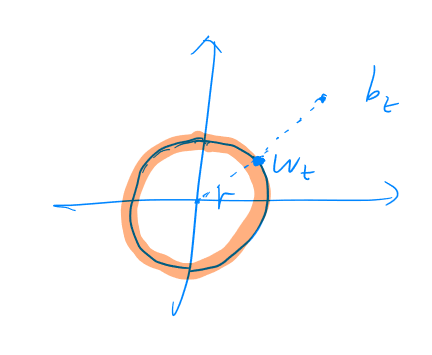
\includegraphics{graph.PNG}
    
    \section{Principal Component Analysis}

\textbf{Example:} \\
Let $ \[
   M=
  \left[ {\begin{array}{ccccc}
   5 & 4 & 3 & 0 & 1\\
   5 & 4 & 3 & 0 & 1\\
  \end{array} } \right]
\]$\\
\\
The values can be projected along x-y axis like:\\
    \includegraphics{graph2.PNG}
\\
These values can be projected on x-axis, allowing us to reduce the dimensionality of M from 2 to 1. Hence,\\
\\$ \[
   M=
  \left[ {\begin{array}{ccccc}
   5 & 4 & 3 & 0 & 1\\
  \end{array} } \right]
\]$\\
\\
However, if noise is present in the data, our matrix will be:\\ 
\\$ \[
   M=
  \left[ {\begin{array}{ccc}
   5+0.001 & 4+10^{-6} & ... \\
   5-0.001 & 4-10^{-5} & ... \\
  \end{array} } \right]
\]$\\
\\
The values can be represented along x-y axis like: \\
\\
\includegraphics{graph3.PNG}
\\
The noise in the above situation create problems for dimensionality reduction and distorts the "underlying structure" of the data and makes it harder to identify linear dependencies in M. Hence, its important to eliminate noise.

\section{Brief overview of Linear algebra}

\textbf{Subspace: $V \subseteq  R^d $}
\begin{enumerate}
    \item{$\vec{0} \in V$: includes the zero vector}
    \item{Closed under linear combination}: $for\,any\,(\vec{u},\vec{v}) \in V$: $  a.\vec{u} + b.\vec{v} \in V$
\end{enumerate}
\\
For a given example vector space V,:\\

$V={a_1\vec{e_1}+a_2\vec{e_2}+a_3\vec{e_3}}$\\
\\$rank = 3,\,dim = 3,\,span(e_1,e_2,e_3)$\\
\\$\therefore\,$ Rank is equivalent to the number of basis vectors\\
\\
\textbf{Linear independence:}\\
\\
For a group of vectors $V= (v_1,v_2,..,v_n)$ are independent when:\\

$a_1.v_1+a_2.v_2+...+a_n.v_n=0$     ..if and only if $a_1=0,a_2=0,...a_n=0$

\section{PCA(contd.)}
\\
We know that clean data is in the form of low-rank data matrix. Hence to remove noise, we try to find a low rank matrix that approximates the observed data.\\
\\
Mathematically,\\

\\minimize $||X - M||_F$ such that $rank(X)<k$       ...(natural form)\\
where,\\$||M||_F=\sqrt{\sum{_i,_j}m^2_{i,j}} \approx ||v_2||$\\
\\
Let's assume the matrix case,\\
$M: R^d$\\$X: R^d$\\

\\$min_X||M-X||_2$ such that $||X||_0 \leq k$
\\
where, $X = H_K(X)$\\
\\
Consider following vector case,\\
$M=(m_1,m_2,...,m_d)$
\\
$= m_1.\left[ {\begin{array}{c}
   1\\
   0\\
   0\\
   ..\\
   0
  \end{array} } \right]$ + 
  m_2.\left[ {\begin{array}{c}
   0\\
   1\\
   0\\
   ..\\
   0
  \end{array} } \right]$ + .... +
  m_d.\left[ {\begin{array}{c}
   0\\
   0\\
   0\\
   ..\\
   1
  \end{array} } \right]$\\
\\
To solve above equation for global optima, we use following steps:
\begin{enumerate}
    \item{Step 1}: decompose $M=\sum m_i.v_i$  where $v_i$ is basis vectors
    \item{Step 2}: select k largest coefficients from $m_1,..,m_d$
    \item{Step 3}: set everything else to zero 
\end{enumerate}
\\
Back to matrix case, we try the above steps:
\begin{enumerate}
    \item{Step 1}: decompose into $M=\sum{i=1}\alpha_i.C_i$  where $C_i$ are matrices orthogonal to each other.\\If you consider step 1 to be a black box that takes M and returns $C_1,..,C_T$ and $\alpha_1,..,\alpha_T$, then that back box is Single value decomposition(SVD)
    \item{Step 2}: select k largest coefficients from $\alpha_1,..,alpha_T$
    \item{Step 3}: set everything else to zero 
\end{enumerate}
\\ The $C_i$ from above discussion can be considered to be a basis vector in the corresponding vector case.
\\ As basis vectors can be represented as linear combination of any vector in subspace.The same holds for matrices too.
\\ So if M is of size $(d\times n)$, $C_i$ is the basis for all $(d\times n)$ matrices.\\
\\
By SVD, we get\\

\\$M \rightarrow \mu \cdot \sum \cdot V$
\\where,\\
\\$M: R^{d \times n}$
\\$\mu: R^{d \times d}$
\\$\sum: R^{d \times n}$
\\$V: R^{n \times n}$
\\and,
\\$u^Tu=uu^T=I$
\\$v^Tv=vv^t=I$
\\in $\sum$ non-diagonal elements are 0
\\
\\From SVD rules, the $min(d^2n,n^2d)$ is guaranteed to return the values for $\mu,\sum,V$. Also from SVD, we have:\\

\\$\sum \cdot V = C_{d\times n}$



\end{document}